\begin{frame}[plain]
   %\begin{columns}
   %   \column{1.2\textwidth}
      \maketitle
   %\end{columns}
\end{frame}

% first frame:
% REAL ROBOTS! REAL-WORLD PROBLEMS!
% overview of manipulation planning problem?
\begin{frame}
   \frametitle{Autonomous Manipulation Tasks}
   \begin{tikzpicture}
      \draw[step=1,black!10,very thin,opacity=\gridopacity] (0,0) grid (12,8);
   
      \node[inner sep=0] at ( 2,5.0) {\includegraphics[width=3.5cm]{images/herb.jpg}};
      \node[inner sep=0] at ( 6,5.0) {\includegraphics[width=3.5cm]{images/arms.jpg}};
      \node[inner sep=0] at (10,5.0) {\includegraphics[width=3.5cm]{images/chimp.jpg}};
      \node at ( 2,2.4) {Herb};
      \node at ( 6,2.4) {ARM-S};
      \node at (10,2.4) {CHIMP};
      
      \begin{scope}[font=\footnotesize]
         \only<2->{
            \node[draw,align=center,minimum height=1.2cm,font=\tiny]
               (a) at (1,0.85) {Unknown\\Environment};
         }
         
         \only<3->{
            \node[fill=blue!10,rounded corners,align=center,minimum height=1.5cm]
               (b) at (3,0.85) {Onboard\\Sensors};
            \draw[->,line width=1pt] (a) -- (b);
         }
         
         \only<4->{
            \node[draw,align=center,minimum height=1.2cm,font=\tiny]
               (c) at (5,0.85) {Geometric\\World\\Model};
            \draw[->,line width=1pt] (b) -- (c);
         }
         
         \only<5->{
            \node[fill=blue!10,rounded corners,align=center,minimum height=1.5cm]
               (d) at (7,0.85) {Onboard\\Motion\\Planner};
            \draw[->,line width=1pt] (c) -- (d);
         }
         
         \only<6->{
            \node[draw,align=center,minimum height=1.2cm,font=\tiny]
               (e) at (9,0.85) {Motion};
               \draw[->,line width=1pt] (d) -- (e);
         }
         
         \only<7->{
            \node[fill=blue!10,rounded corners,align=center,minimum height=1.5cm]
               (f) at (11,0.85) {Motion\\Execution};
            \draw[->,line width=1pt] (e) -- (f);
         }
      \end{scope}
   
   \end{tikzpicture}
\end{frame}

\begin{frame}
   \frametitle{Example Manipulation Tasks}
   \begin{tikzpicture}
      \draw[step=1,black!10,very thin,opacity=\gridopacity] (0,0) grid (12,8);

      \fill[black!80] (0.1,3.0) rectangle (11.9,6.6);

      \node[fill=black,inner sep=1pt] at (3.1,4.8) {
         \movie[width=5.333333cm,height=3.00cm,
            loop,autostart]{}{chimp-trials-debris-fast.mp4}
      };
      
      \node[fill=black,inner sep=1pt] at (8.9,4.8) {
         \movie[width=5.333333cm,height=3.00cm,
            loop,autostart]{}{herb-tableclear-2-fast.mp4}
      };

      %\node[fill=black,inner sep=1pt] at (3,6.3) {
      %   \movie[width=5.333333cm,height=3.00cm,
      %      loop,autostart]{}{chimp-trials-debris-fast.mp4}
      %};
      
      %\node[fill=black,inner sep=1pt] at (9,6.3) {
      %   \movie[width=5.333333cm,height=3.00cm,
      %      loop,autostart]{}{herb-tableclear-2-fast.mp4}
      %};
      
      %\node[fill=black,minimum width=4cm, minimum height=3cm,text=white] at (3,3.2) {
      %   ARM-S Example?
      %};
      
      %\node[fill=black,minimum width=4cm, minimum height=3cm,text=white] at (9,3.2) {
      %   Other (PR-2) Example?
      %};
   
      %\hyperlinkmovie[play]{mylabel}{play}

      \begin{scope}[font=\footnotesize]
         \node[draw,align=center,minimum height=1.2cm,font=\tiny]
            (a) at (1,0.85) {Unknown\\Environment};
         \node[fill=blue!10,rounded corners,align=center,minimum height=1.5cm]
            (b) at (3,0.85) {Onboard\\Sensors};
         \draw[->,line width=1pt] (a) -- (b);
         \node[draw,align=center,minimum height=1.2cm,font=\tiny]
            (c) at (5,0.85) {Geometric\\World\\Model};
         \draw[->,line width=1pt] (b) -- (c);
         \only<1>{
            \node[fill=blue!10,rounded corners,align=center,minimum height=1.5cm]
               (d) at (7,0.85) {Onboard\\Motion\\Planner};
         }
         \only<2>{
            \node[fill=green!50,rounded corners,align=center,minimum height=1.5cm]
               (d) at (7,0.85) {Onboard\\Motion\\Planner};
         }
         \draw[->,line width=1pt] (c) -- (d);
         \node[draw,align=center,minimum height=1.2cm,font=\tiny]
            (e) at (9,0.85) {Motion};
            \draw[->,line width=1pt] (d) -- (e);
         \node[fill=blue!10,rounded corners,align=center,minimum height=1.5cm]
            (f) at (11,0.85) {Motion\\Execution};
         \draw[->,line width=1pt] (e) -- (f);
      \end{scope}

   \end{tikzpicture}
\end{frame}

%\begin{frame}
%   \frametitle{tasks are slow because planning is slow}
%   
%   Make figure:
%   \begin{tabular}{ll}
%      HERB pic & 50\% planning time, 50\% exec time \\
%      CHIMP pic & 40\% planning time, 60\% exec time \\
%   \end{tabular}
%   
%   \medskip
%   Focus on planning for manipulation tasks.
%   Talk about WHY planning is slow, and WHY planning is necesary
%   in these problems.
%   
%   \medskip
%   Do I need this slide?
%\end{frame}

\begin{frame}
   \frametitle{3 Challenges to Efficient Manipulation Planning}
   \begin{tikzpicture}
      \draw[step=1,black!10,very thin,opacity=\gridopacity] (0,0) grid (12,8);

   \node[inner sep=0pt] at (6,5.3) {%
      \only<1-2>{\includegraphics[width=11.5cm]{figs/herb-fridge-a.png}}%
      \only<3>{\includegraphics[width=11.5cm]{figs/herb-fridge-b.png}}%
      \only<4>{\includegraphics[width=11.5cm]{figs/herb-fridge-c.png}}%
      \only<5>{\includegraphics[width=11.5cm]{figs/herb-fridge-a.png}}%
   };

   % figure adapted from proposal doc
   \begin{scope}[font=\scriptsize,shift={(1.5,1.5)}]
      
      % root sets
      \only<3->{
         \node[draw,black,rounded corners,minimum height=1.5cm,minimum width=1cm]
            (Xgrasp) at (3,0) {};
         \node[above=0cm of Xgrasp] {Grasp};
      }
      \only<4->{
         \node[draw,black,rounded corners,minimum height=1.5cm,minimum width=1cm]
            (Xdrop) at (6,0) {};
         \node[above=0cm of Xdrop] {Place};
      }
      
      % nodes
      \only<2->
      {
         \node[circle,fill=black,inner sep=2] (xstart) at (0,0) {};
         \node[above=0.1cm of xstart] {$q_{\mbox{\scriptsize start}}$};
      }
      %\node[circle,fill=black,inner sep=2] (xg1) at (2.8,0.5) {};
      %\node[circle,fill=black,inner sep=2] (xg2) at (3.1,0.1) {};
      \only<3->{
         \node[circle,fill=black,inner sep=2] (xg3) at (2.9,-0.5) {};
      }
      \only<4->{
         \node[circle,fill=black,inner sep=2] (xd1) at (5.9,0.3) {};
      }
      %\node[circle,fill=black,inner sep=2] (xd2) at (6.0,-0.4) {};
      \only<5->
      {
         \node[circle,fill=black,inner sep=2] (xend) at (9,0) {};
         \node[above=0.1cm of xend] {$q_{\mbox{\scriptsize end}}$};
      }
      
      \only<3->{
         % in S1
         %\draw[line width=1.5mm,white]
         %   (xstart) .. controls (1,0.2) and (1.4,0.9) .. (xg1);
         %\draw[line width=1.5mm,white]
         %   (xstart) .. controls (1.5,0.2) .. (xg2);
         \draw[line width=1.5mm,white]
            (xstart) .. controls (1.8,-0.6) and (1.6,-0.8) .. (xg3);
         %\draw
         %   (xstart) .. controls (1,0.2) and (1.4,0.9) .. (xg1);
         %\draw
         %   (xstart) .. controls (1.5,0.2) .. (xg2);
         \draw
            (xstart) .. controls (1.8,-0.6) and (1.6,-0.8) .. (xg3);
      }
      
      \only<4->{
         % in s2
         %\draw[line width=1.5mm,white]
         %   (xg1) -- (4.7,0.6);
         %\draw[line width=1.5mm,white]
         %   (xg2) .. controls (4.5,1) and (3.5,-1.2) .. (4.5,-0.4)
         %         .. controls (5.5,0.5) and (5.0,-1.3) .. (xd2);
         %\draw
         %   (xg1) -- (4.7,0.6);
         %\draw
         %   (xg2) .. controls (4.5,1) and (3.5,-1.2) .. (4.5,-0.4)
         %         .. controls (5.5,0.5) and (5.0,-1.3) .. (xd2);
         \draw[line width=1.5mm,white]
            (xg3) .. controls (4.3, 0.2) and (4.5,-0.2) .. (xd1);
         \draw
            (xg3) .. controls (4.3, 0.2) and (4.5,-0.2) .. (xd1);
      }
      
      \only<5->{
         % in s3
         \draw[line width=1.5mm,white]
            (xd1) .. controls (8,0.3) and (8,0.1) .. (xend);
         \draw
            (xd1) .. controls (8,0.3) and (8,0.1) .. (xend);
      }
      
      \only<3->{
         \node[fill,black,rounded corners,minimum height=1.5cm,minimum width=1cm,
            opacity=0.1] at (3,0) {};
      }
      \only<4->{
         \node[fill,black,rounded corners,minimum height=1.5cm,minimum width=1cm,
            opacity=0.1] at (6,0) {};
      }
      
      %\draw [decorate,decoration={brace,mirror,amplitude=5pt}]
      %(0.0,-0.9) -- (2.9,-0.9) node [black,midway,yshift=-0.4cm,align=center]
      %   {bottle in fridge};

      %\draw [decorate,decoration={brace,mirror,amplitude=5pt}]
      %(3.1,-0.9) -- (5.9,-0.9) node [black,midway,yshift=-0.4cm,align=center]
      %   {bottle in hand};

      %\draw [decorate,decoration={brace,mirror,amplitude=5pt}]
      %(6.1,-0.9) -- (9.0,-0.9) node [black,midway,yshift=-0.4cm,align=center]
      %   {bottle on tray};
   \end{scope}

   %\node[inner sep=0pt] at (6,2.25) {
   %   \includegraphics{build/intro-subprob-cspace}
   %};
   
   %In order to describe why it's so slow,
   %I need to talk a bit about the problem's structure
   %and current approaches to handling it.
   %
   %I will be using this HERB example (removing items from a fridge)
   %throughout the talk.
   %
   %Below, show a 2D diagram of three steps of this plan,
   %which I then reference in the next three challenge slides.
   
   \end{tikzpicture}
\end{frame}

\begin{frame}
   \frametitle{Challenge 1: The Planning vs. Execution Tradeoff}
   \begin{tikzpicture}
      \draw[step=1,black!10,very thin,opacity=\gridopacity] (0,0) grid (12,8);

   \node[inner sep=0pt] at (3,5.3) {%
      \includegraphics[width=5.75cm]{figs/herb-fridge-a-skinny.png}
   };

   \only<3->{
      \node[fill=black!5,rounded corners,font=\small,anchor=north] at (9,7.5)
         {\begin{minipage}{5.5cm}

            Configuration space $\mathcal{C}$ is:
            \only<4->{
               \begin{itemize}[leftmargin=*,itemsep=0pt,topsep=2pt]
               \item continuous
               \only<5->{\item high-dimensional}
               \end{itemize}
            }
         
            \only<7->{
               \medskip
               Valid subset $\mathcal{C}_{\ms{free}}$ is:
            }
            \only<8->{
               \begin{itemize}[leftmargin=*,itemsep=0pt,topsep=2pt]
               \item induced by complex geometry
               \only<9->{\item expensive to validate motions}
               \end{itemize}
            }
            
            \only<10->{
               \begin{center}
                  {\bf Planning is expensive!}
               \end{center}
            }
            
         \end{minipage}};
   }
   
   \only<11->{
      \node[fill=blue!10,rounded corners,font=\small,anchor=north] at (9,3)
         {\begin{minipage}{5.5cm}
            \begin{center}
            For manipulation tasks,\\
            planning effort $\approx$ execution effort
            \end{center}
         \end{minipage}};
   }
   
   \only<12->{
      \node[fill=blue!10,rounded corners,font=\small,anchor=north] at (9,1.75)
         {\begin{minipage}{5.5cm}
            \begin{center}
            Robot's effort spent planning
            detracts directly from available
            task resource budget.
            \end{center}
         \end{minipage}};
   }

   % figure adapted from proposal doc
   \begin{scope}[font=\scriptsize,shift={(1.5,1.5)}]
      
      % root sets
      \node[draw,black,rounded corners,minimum height=1.5cm,minimum width=1cm]
         (Xgrasp) at (3,0) {};
      \node[above=0cm of Xgrasp] {Grasp};
      
      % cspace sets (lines only)
      \only<2->{
         \node[draw,black,rounded corners,minimum height=1.8cm,minimum width=1.8cm,dashed]
            (S1) at (1.5,0) {};
         \node[above left=-0.7cm of S1] {$\mathcal{C}$};
      }
      
      % nodes
      \node[circle,fill=black,inner sep=2] (xstart) at (0,0) {};
      \node[above=0.1cm of xstart] {$q_{\mbox{\scriptsize start}}$};
      \node[circle,fill=black,inner sep=2] (xg3) at (2.9,-0.5) {};
      
      % in S1
      \draw[line width=1.5mm,white]
         (xstart) .. controls (1.8,-0.6) and (1.6,-0.8) .. (xg3);
      
      % draw s1 cfree
      \only<6->{
         \begin{scope}[even odd rule]
            \clip[rounded corners] (0.61,-0.89) rectangle (2.39,0.89);
            \clip[rotate around={10:(1.1,0.5)}] (-3,-3) rectangle (3,3)
                     (0.6,-0.0) rectangle (1.6,1.0);
            \fill[blue!15,rotate around={-15:(1.5,-0.5)}] (1.5,-0.5) ellipse (1.4cm and 0.5cm);
            \fill[blue!15,rotate around={-25:(1.5, 1.0)}] (1.5, 1.0) ellipse (1.4cm and 0.5cm);
         \end{scope}
         \node[draw,inner sep=0,fill=blue!20,minimum width=0.5cm,minimum height=0.2cm]
            (Cfreebox1) at (1.2, -1.2) {};
         \node[right=0cm of Cfreebox1] {: $\mathcal{C}_{\mbox{\tiny free}}$}; 
      }
         
      \draw
         (xstart) .. controls (1.8,-0.6) and (1.6,-0.8) .. (xg3);
      
      \node[fill,black,rounded corners,minimum height=1.5cm,minimum width=1cm,
         opacity=0.1] at (3,0) {};
      
      %\draw [decorate,decoration={brace,mirror,amplitude=5pt}]
      %(0.0,-0.9) -- (2.9,-0.9) node [black,midway,yshift=-0.4cm,align=center]
      %   {bottle in fridge};

      %\draw [decorate,decoration={brace,mirror,amplitude=5pt}]
      %(3.1,-0.9) -- (5.9,-0.9) node [black,midway,yshift=-0.4cm,align=center]
      %   {bottle in hand};

      %\draw [decorate,decoration={brace,mirror,amplitude=5pt}]
      %(6.1,-0.9) -- (9.0,-0.9) node [black,midway,yshift=-0.4cm,align=center]
      %   {bottle on tray};
   \end{scope}

   \end{tikzpicture}
\end{frame}

\begin{frame}
   \frametitle{Challenge 2: Incongruent Steps Impede Reuse}
   \begin{tikzpicture}
      \draw[step=1,black!10,very thin,opacity=\gridopacity] (0,0) grid (12,8);

   \node[inner sep=0pt] at (3,5.3) {%
      \only<1>{\includegraphics[width=5.75cm]{figs/herb-fridge-b-skinny.png}}%
      \only<2->{\includegraphics[width=5.75cm]{figs/herb-fridge-c-skinny.png}}%
   };

   \only<5->{
      \node[fill=black!5,rounded corners,font=\small,anchor=north] at (9,7.5)
         {\begin{minipage}{5.5cm}
            $\mathcal{C}_{\ms{free}}$ is dependent on:
            \begin{itemize}[leftmargin=*,itemsep=0pt,topsep=2pt]
               \item distribution of all obstacles
               \item grasp pose of held objects
               \item robot location
            \end{itemize}
         \end{minipage}};
   }
   
   \only<6->{
      \node[fill=blue!10,rounded corners,font=\small,anchor=north] at (9,5.3)
         {\begin{minipage}{5.5cm}
            \begin{center}
            For manipulation tasks,\\
            this subset changes at \emph{every} step!
            \end{center}
         \end{minipage}};
   }
   
   \only<7->{
      \node[fill=blue!10,rounded corners,font=\small,anchor=north] at (9,4.1)
         {\begin{minipage}{5.5cm}
            \begin{center}
            How can we reuse precious planning computation?
            \end{center}
         \end{minipage}};
   }

   % figure adapted from proposal doc
   \begin{scope}[font=\scriptsize,shift={(1.5,1.5)}]
      
      % root sets
      \node[draw,black,rounded corners,minimum height=1.5cm,minimum width=1cm]
         (Xgrasp) at (3,0) {};
      \node[above=0cm of Xgrasp] {Grasp};
      
      \only<3->{
         \node[draw,black,rounded corners,minimum height=1.5cm,minimum width=1cm]
            (Xdrop) at (6,0) {};
         \node[above=0cm of Xdrop] {Place};
      }
      
      % cspace sets
      \node[draw,black,rounded corners,minimum height=1.8cm,minimum width=1.8cm,dashed]
         (S1) at (1.5,0) {};
      \node[above left=-0.7cm of S1] {$\mathcal{C}$};
      
      \only<4->{
         \node[draw,black,rounded corners,minimum height=1.8cm,minimum width=1.8cm,dashed]
            (S1) at (4.5,0) {};
         \node[above left=-0.7cm of S1] {$\mathcal{C}$};
      }
      
      % nodes
      \node[circle,fill=black,inner sep=2] (xstart) at (0,0) {};
      \node[above=0.1cm of xstart] {$q_{\mbox{\scriptsize start}}$};
      \node[circle,fill=black,inner sep=2] (xg3) at (2.9,-0.5) {};
      
      % in S1
      \draw[line width=1.5mm,white]
         (xstart) .. controls (1.8,-0.6) and (1.6,-0.8) .. (xg3);
      % draw s1 cfree
      \begin{scope}[even odd rule]
         \clip[rounded corners] (0.61,-0.89) rectangle (2.39,0.89);
         \clip[rotate around={10:(1.1,0.5)}] (-3,-3) rectangle (3,3)
                  (0.6,-0.0) rectangle (1.6,1.0);
         \fill[blue!15,rotate around={-15:(1.5,-0.5)}] (1.5,-0.5) ellipse (1.4cm and 0.5cm);
         \fill[blue!15,rotate around={-25:(1.5, 1.0)}] (1.5, 1.0) ellipse (1.4cm and 0.5cm);
      \end{scope}
      \node[draw,inner sep=0,fill=blue!20,minimum width=0.5cm,minimum height=0.2cm]
            (Cfreebox1) at (1.2, -1.2) {};
         \node[right=0cm of Cfreebox1] {: $\mathcal{C}_{\mbox{\tiny free1}}$}; 
      \draw
         (xstart) .. controls (1.8,-0.6) and (1.6,-0.8) .. (xg3);
      
      % in s2
      \only<3->{
         \node[circle,fill=black,inner sep=2] (xd1) at (5.9,0.3) {};
         \draw[line width=1.5mm,white]
            (xg3) .. controls (4.3, 0.2) and (4.5,-0.2) .. (xd1);
         \only<4->{
            % draw s2 cfree
            \begin{scope}[even odd rule]
               \clip[rounded corners] (3.61,-0.89) rectangle (5.39,0.89);
               \clip[rotate around={10:(4.1,0.5)}] (0,-3) rectangle (6,3)
                     (3.6,-0.0) rectangle (4.6,1.0);
               \fill[red!15,rotate around={15:(4.5,-0.2)}] (4.5,-0.2) ellipse (1.4cm and 0.5cm);
            \end{scope}
            \node[draw,inner sep=0,fill=red!20,minimum width=0.5cm,minimum height=0.2cm]
               (Cfreebox1) at (4.2, -1.2) {};
            \node[right=0cm of Cfreebox1] {: $\mathcal{C}_{\mbox{\tiny free2}}$};
         }
         \draw
            (xg3) .. controls (4.3, 0.2) and (4.5,-0.2) .. (xd1);
      }
      
      \node[fill,black,rounded corners,minimum height=1.5cm,minimum width=1cm,
         opacity=0.1] at (3,0) {};
      \only<3->{
         \node[fill,black,rounded corners,minimum height=1.5cm,minimum width=1cm,
            opacity=0.1] at (6,0) {};
      }
      
      %\draw [decorate,decoration={brace,mirror,amplitude=5pt}]
      %(0.0,-0.9) -- (2.9,-0.9) node [black,midway,yshift=-0.4cm,align=center]
      %   {bottle in fridge};

      %\draw [decorate,decoration={brace,mirror,amplitude=5pt}]
      %(3.1,-0.9) -- (5.9,-0.9) node [black,midway,yshift=-0.4cm,align=center]
      %   {bottle in hand};

      %\draw [decorate,decoration={brace,mirror,amplitude=5pt}]
      %(6.1,-0.9) -- (9.0,-0.9) node [black,midway,yshift=-0.4cm,align=center]
      %   {bottle on tray};
   \end{scope}

   \end{tikzpicture}
\end{frame}

\begin{frame}
   \frametitle{Challenge 3: Coupled Steps Require Planning Ahead}
   \begin{tikzpicture}
      \draw[step=1,black!10,very thin,opacity=\gridopacity] (0,0) grid (12,8);

   \node[inner sep=0pt] at (3,5.3) {%
      \only<1->{\includegraphics[width=5.75cm]{figs/herb-fridge-a-skinny.png}}%
      %\only<2->{\includegraphics[width=5.75cm]{figs/herb-fridge-d-skinny.png}}%
   };

   \only<2->{
      \node[fill=black!5,rounded corners,font=\small,anchor=north] at (9,7.7)
         {\begin{minipage}{5.5cm}
            Each step admits several choices:
            \begin{itemize}[leftmargin=*,itemsep=0pt,topsep=2pt]
               \item which object
               \item which grasp/placement
               \item which IK solution
            \end{itemize}
         \end{minipage}};
   }
   
   \only<3->{
      \node[fill=blue!10,rounded corners,font=\small,anchor=north] at (9,5.5)
         {\begin{minipage}{5.5cm}
            \begin{center}
            For manipulation tasks,\\
            a bad choice can render ensuing steps \emph{impossible}
            \only<-4>{\color{blue!10}or \emph{difficult}.}%
            \only<5->{or \emph{difficult}.}%
            \end{center}
         \end{minipage}};
   }
   
   \only<10->{
      \node[fill=blue!10,rounded corners,font=\small,anchor=north] at (9,3.9)
         {\begin{minipage}{5.5cm}
            \begin{center}
            This magnifies the need for efficient motion planning.
            \end{center}
         \end{minipage}};
   }

   % figure adapted from proposal doc
   \begin{scope}[font=\scriptsize,shift={(1.5,1.5)}]
      
      % root sets
      \node[draw,black,rounded corners,minimum height=1.5cm,minimum width=1cm]
         (Xgrasp) at (3,0) {};
      \node[above=0cm of Xgrasp] {Grasp};
      \node[draw,black,rounded corners,minimum height=1.5cm,minimum width=1cm]
         (Xdrop) at (6,0) {};
      \node[above=0cm of Xdrop] {Place};
      
      % nodes
      \node[circle,fill=black,inner sep=2] (xstart) at (0,0) {};
      \node[above=0.1cm of xstart] {$q_{\mbox{\scriptsize start}}$};
      
      \only<2->{
         % grasp choices
         \node[circle,fill=black,inner sep=2] (xg1) at (2.8,0.5) {};
         \node[circle,fill=black,inner sep=2] (xg2) at (3.1,0.1) {};
         \node[circle,fill=black,inner sep=2] (xg3) at (2.9,-0.5) {};
         % place choices
         \node[circle,fill=black,inner sep=2] (xd1) at (5.9,0.3) {};
         \node[circle,fill=black,inner sep=2] (xd2) at (6.0,-0.4) {};
         % xend 
         \node[circle,fill=black,inner sep=2] (xend) at (9,0) {};
         \node[above=0.1cm of xend] {$q_{\mbox{\scriptsize end}}$};
      }
      
      %\only<2->{
      %   
      %}
      
      % in S1
      \only<3->{
         \draw[line width=1.5mm,white]
            (xstart) .. controls (1,0.2) and (1.4,0.9) .. (xg1);
      }
      \only<5->{
         \draw[line width=1.5mm,white]
            (xstart) .. controls (1.5,0.2) .. (xg2);
      }
      \only<7->{
         \draw[line width=1.5mm,white]
            (xstart) .. controls (1.8,-0.6) and (1.6,-0.8) .. (xg3);
      }
      \only<3->{
         \draw
            (xstart) .. controls (1,0.2) and (1.4,0.9) .. (xg1);
      }
      \only<5->{
         \draw
            (xstart) .. controls (1.5,0.2) .. (xg2);
      }
      \only<7->{
         \draw
            (xstart) .. controls (1.8,-0.6) and (1.6,-0.8) .. (xg3);
      }
      
      % in s2
      \only<4->{
         \draw[line width=1.5mm,white]
            (xg1) -- (4.7,0.6);
         \draw
            (xg1) -- (4.7,0.6);
      }
      \only<6->{
         \draw[line width=1.5mm,white]
            (xg2) .. controls (4.5,1) and (3.5,-1.2) .. (4.5,-0.4)
                  .. controls (5.5,0.5) and (5.0,-1.3) .. (xd2);
         \draw
            (xg2) .. controls (4.5,1) and (3.5,-1.2) .. (4.5,-0.4)
                  .. controls (5.5,0.5) and (5.0,-1.3) .. (xd2);
      }
      
      \only<8->{
         \draw[line width=1.5mm,white]
            (xg3) .. controls (4.3, 0.2) and (4.5,-0.2) .. (xd1);
         \draw
            (xg3) .. controls (4.3, 0.2) and (4.5,-0.2) .. (xd1);
      }
      
      \only<9->{
         % in s3
         \draw[line width=1.5mm,white]
            (xd1) .. controls (8,0.3) and (8,0.1) .. (xend);
         \draw
            (xd1) .. controls (8,0.3) and (8,0.1) .. (xend);
      }
      
      \node[fill,black,rounded corners,minimum height=1.5cm,minimum width=1cm,
         opacity=0.1] at (3,0) {};
      \node[fill,black,rounded corners,minimum height=1.5cm,minimum width=1cm,
         opacity=0.1] at (6,0) {};
      
   \end{scope}

   \end{tikzpicture}
\end{frame}

\begin{frame}
   \frametitle{Objective of Proposed Work}
   \begin{tikzpicture}
      \draw[step=1,black!10,very thin,opacity=\gridopacity] (0,0) grid (12,8);
   
      % figure adapted from proposal doc
      \begin{scope}[font=\scriptsize,shift={(1.5,6.25)}]
         
         % root sets
         \node[draw,black,rounded corners,minimum height=1.5cm,minimum width=1cm]
            (Xgrasp) at (3,0) {};
         \node[above=0cm of Xgrasp] {Grasp};
         \node[draw,black,rounded corners,minimum height=1.5cm,minimum width=1cm]
            (Xdrop) at (6,0) {};
         \node[above=0cm of Xdrop] {Place};
         
         % nodes
         \node[circle,fill=black,inner sep=2] (xstart) at (0,0) {};
         \node[above=0.1cm of xstart] {$q_{\mbox{\scriptsize start}}$};
         
         % grasp choices
         \node[circle,fill=black,inner sep=2] (xg1) at (2.8,0.5) {};
         \node[circle,fill=black,inner sep=2] (xg2) at (3.1,0.1) {};
         \node[circle,fill=black,inner sep=2] (xg3) at (2.9,-0.5) {};
         % place choices
         \node[circle,fill=black,inner sep=2] (xd1) at (5.9,0.3) {};
         \node[circle,fill=black,inner sep=2] (xd2) at (6.0,-0.4) {};
         % xend 
         \node[circle,fill=black,inner sep=2] (xend) at (9,0) {};
         \node[above=0.1cm of xend] {$q_{\mbox{\scriptsize end}}$};
         
         \draw[line width=1.5mm,white]
            (xstart) .. controls (1,0.2) and (1.4,0.9) .. (xg1);
         \draw[line width=1.5mm,white]
            (xstart) .. controls (1.5,0.2) .. (xg2);
         \draw[line width=1.5mm,white]
            (xstart) .. controls (1.8,-0.6) and (1.6,-0.8) .. (xg3);
         \draw
            (xstart) .. controls (1,0.2) and (1.4,0.9) .. (xg1);
         \draw
            (xstart) .. controls (1.5,0.2) .. (xg2);
         \draw
            (xstart) .. controls (1.8,-0.6) and (1.6,-0.8) .. (xg3);
         \draw[line width=1.5mm,white]
            (xg1) -- (4.7,0.6);
         \draw
            (xg1) -- (4.7,0.6);
         \draw[line width=1.5mm,white]
            (xg2) .. controls (4.5,1) and (3.5,-1.2) .. (4.5,-0.4)
                  .. controls (5.5,0.5) and (5.0,-1.3) .. (xd2);
         \draw
            (xg2) .. controls (4.5,1) and (3.5,-1.2) .. (4.5,-0.4)
                  .. controls (5.5,0.5) and (5.0,-1.3) .. (xd2);
         \draw[line width=1.5mm,white]
            (xg3) .. controls (4.3, 0.2) and (4.5,-0.2) .. (xd1);
         \draw
            (xg3) .. controls (4.3, 0.2) and (4.5,-0.2) .. (xd1);
         % in s3
         \draw[line width=1.5mm,white]
            (xd1) .. controls (8,0.3) and (8,0.1) .. (xend);
         \draw
            (xd1) .. controls (8,0.3) and (8,0.1) .. (xend);
         
         \node[fill,black,rounded corners,minimum height=1.5cm,minimum width=1cm,
            opacity=0.1] at (3,0) {};
         \node[fill,black,rounded corners,minimum height=1.5cm,minimum width=1cm,
            opacity=0.1] at (6,0) {};
         
      \end{scope}
   
   
      \node[anchor=north] at (6,5) {\begin{minipage}{11.5cm}
         Planning for manipulation tasks poses three challenges:
         
         \begin{itemize}
         \item Challenge 1: Planning each step is expensive.
         \item Challenge 2: Incongruent steps impede reuse.
         \item Challenge 3: Coupled steps require long planning horizons.
         \end{itemize}
      \end{minipage}};
   
      \node[fill=blue!10,rounded corners] at (6,1.5) {\begin{minipage}{10cm}\centering
         The proposed work is a framework to address\\
         planning for multi-step manipulation tasks \emph{efficiently}.
      \end{minipage}};
   
   \end{tikzpicture}
\end{frame}
